% !TEX root = ../main.tex
% Хавсралт Б

\chapter{Өгөгдөл боловсруулалтын жишээ}
\label{AppendixB}
\pagecolor{white}

Энэ хавсралтад сургалтын өмнөх дүрс боловсруулалтын үндсэн алхмуудыг үзүүлэв. Өгөгдөл нэмэгдүүлэх шатанд эргүүлэх, толин тусгал үүсгэх, гэрэлтэлтийн өөрчлөлт хийх зэрэг аргуудыг ашигласан. (Зургуудыг \texttt{appendix\_scripts/gen\_B\_preprocessing.py} script-ээр үүсгэнэ.)

\begin{figure}[H]
    \centering
    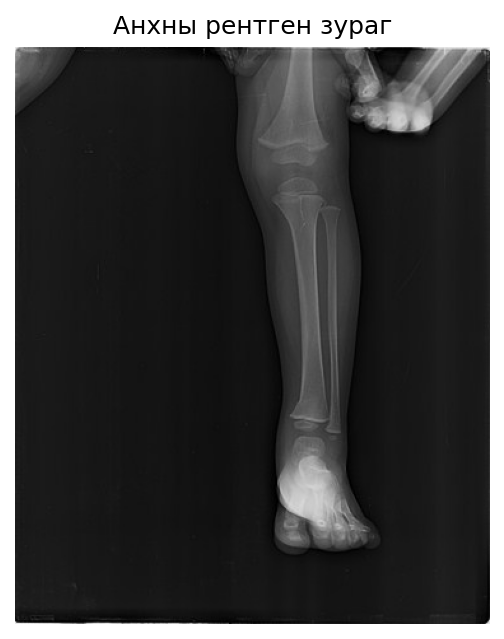
\includegraphics[width=0.45\textwidth,height=0.54\textheight,keepaspectratio]{Figures/appx_b1_original.png}
    \figcaption{Анхны рентген зураг}{Анхны рентген зураг}
    \label{fig:appB_original}
\end{figure}

\begin{figure}[H]
    \centering
    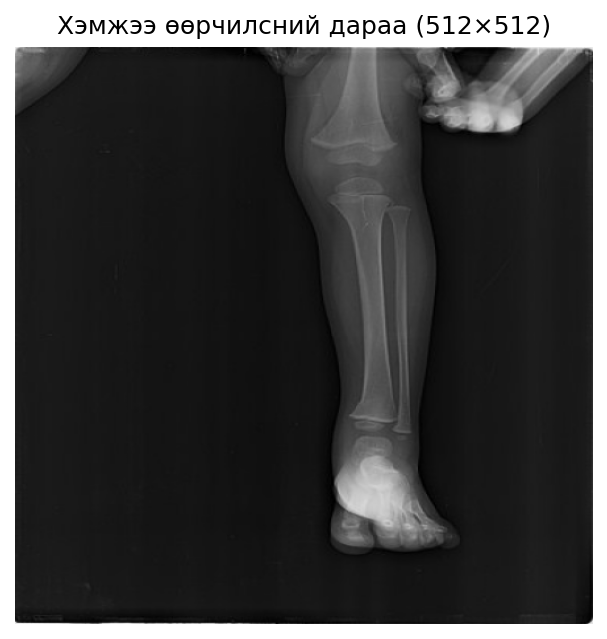
\includegraphics[width=0.45\textwidth,height=0.54\textheight,keepaspectratio]{Figures/appx_b2_resized.png}
    \figcaption{Хэмжээ өөрчилсний дараах зураг}{Хэмжээ өөрчилсний дараах зураг}
    \label{fig:appB_resize}
\end{figure}

\begin{figure}[H]
    \centering
    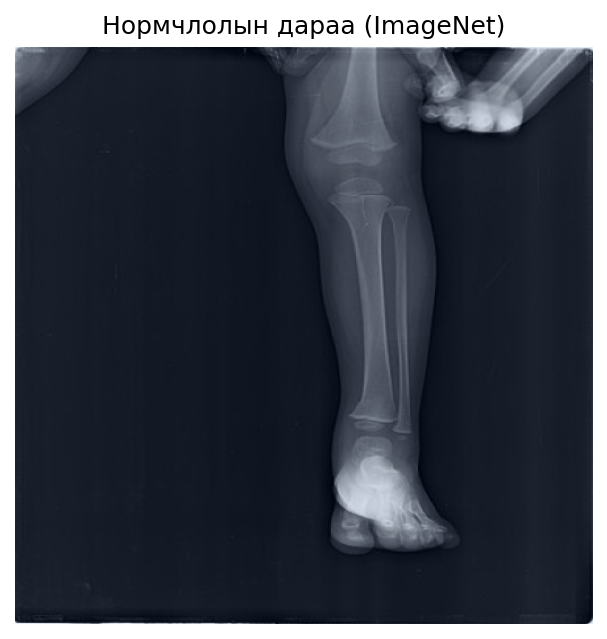
\includegraphics[width=0.45\textwidth,height=0.54\textheight,keepaspectratio]{Figures/appx_b3_normalized.png}
    \figcaption{Нормчлол хийсний дараах зураг}{Нормчлол хийсний дараах зураг}
    \label{fig:appB_norm}
\end{figure}

\begin{figure}[H]
    \centering
    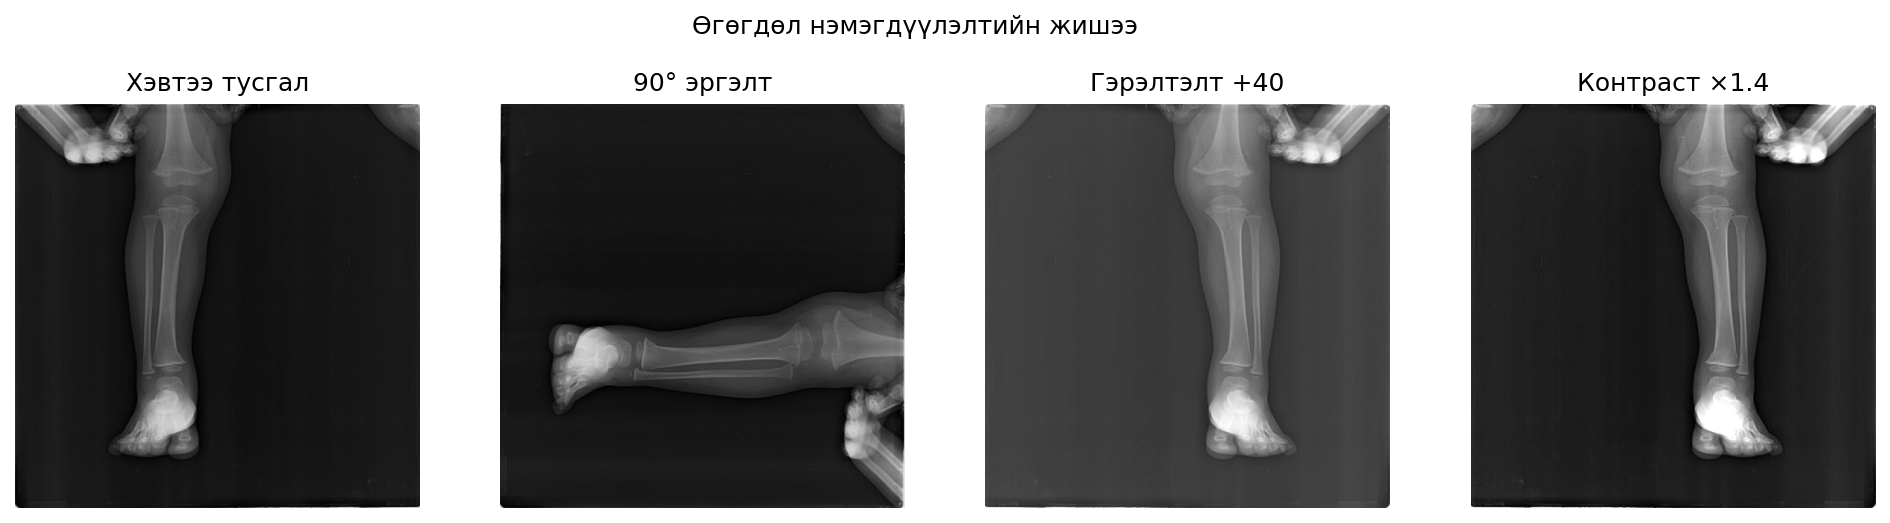
\includegraphics[width=0.82\textwidth,height=0.38\textheight,keepaspectratio]{Figures/appx_b4_augment.png}
    \figcaption{Өгөгдөл нэмэгдүүлэлтийн жишээ}{Өгөгдөл нэмэгдүүлэлтийн жишээ}
    \label{fig:appB_aug}
\end{figure}
